\documentclass[a4paper,11pt]{article}
\usepackage[margin=2cm]{geometry}
\usepackage{graphicx}
\usepackage{color, colortbl}
\usepackage{cite}
\usepackage{url}
\usepackage{float}
\usepackage{arydshln}
\usepackage{pdfpages}
\usepackage{csvsimple}
\usepackage{listings}
\usepackage{algpseudocode}
\usepackage{longtable}
\usepackage{pdflscape}
\usepackage{indentfirst}
\usepackage{mathtools}
\usepackage{amsmath}
\usepackage{amssymb}
\usepackage{tikz}

\definecolor{Green}{rgb}{0.6,1,0.6}
\definecolor{Amber}{rgb}{1,1,0.4}
\definecolor{Red}{rgb}{1,0.6,0.6}

\setlength\parindent{24pt}

\usepackage{fancyhdr}


\title{Some Intuition about Activation Functions in Feed-Forward Neural Networks}


\begin{document}

\maketitle

\abstract
{
Everyone thought it was great to use differentiable, symmetric, non-linear activation functions in feed-forward neural networks, until Alex Krizhevsky \cite{krizhevsky} found that Rectifier Linear Units, despite being not entirely differentiable, nor symmetric, and most of all, piece-wise linear, were computationally cheaper and worth the trade-off with their more sophisticated counterparts. Here are just a few thoughts on why we might care about the shape of the sigmoid and hyperbolic tangent functions, what the implications of using ReLUs are, and possible ways of applying these insights for better learning strategies.
}

\clearpage

\section{Models of Neurons}

The rectified linear unit is the building block for current state-of-the-art implementations of deep convolutional neural networks. In order to bring out its specific characteristics, we shall first consider two other compatible neuron models: the binary threshold neuron, which is the most intuitive, and the logistic sigmoid neuron, which is the most analytically appealing. \\

\paragraph{Binary Threshold Neuron}
\begin{equation}
y = \begin{cases} 1 & \mbox{if } M <= b + \sum\limits_{i=1}^k x_{i}\cdot w_{i}  \text{ , where } M \text{ is a threshold parameter} \\ 
				  0 & \mbox{otherwise} \end{cases}
\end{equation}

Intuitively, $y$ takes a hard decision, just like biological neurons: either a charge is sent, or it isn't. $y$ can be seen as producing spikes, $x_i$ as the indicator value of some feature, and $w_i$ as a parameter of the function that indicates how important $x_i$ is in determining $y$. Although this model is closer than most most to reality, the function is not differentiable, which makes it impossible to use greedy local optimisation learning algorithms - such as gradient descent - which need to compute derivatives involving the activation functions.

\paragraph{Logistic Sigmoid Neuron} 
\begin{equation}
\label{sigmoid neuron}
y = \frac{1}{1 + e^{-z}} \text{, where } z = b + \sum\limits_{i=1}^k x_{i}\cdot w_{i}
\end{equation}

Like the binary threshold neuron, the output domain of this neuron is bounded by 0 and 1. But this time, the function is fully differentiable. Moreover, it is non-linear, which helps to increase performance \cite{DL-book}.

\begin{figure}[h!]
	\centering
	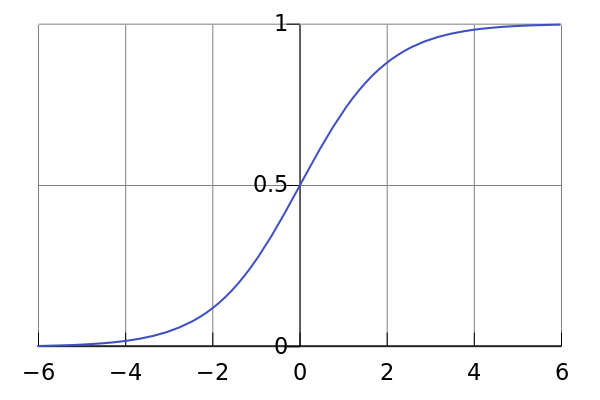
\includegraphics[scale=0.3]{images/sigmoid.png}
	\caption{Single-Input Logistic Sigmoid Neuron}
\end{figure}
 
To see why, the graph plot below lends itself to the following intuition: consider the neuron as a feature detector, where the input x is the amount of evidence for a certain feature, and y is the probability that the feature is present. y is strictly increasing in x, because every extra amount of evidence for the feature increases the probability of its presence. y is bounded above by 1 and 0, because it is a probability. Interestingly, the slope of y is highest in absolute value around $x=0.5$, and tends towards 0 as x departs from 0.5 in either direction. This is like saying: if I'm clueless as to whether the feature is present or not, any evidence in favour of presence or absence will push me easily in that direction; however, the more you want to convince me of it, the higher the required evidence gets.


A disadvantage of this neuron model is that it is computationally expensive to compute.
                
\paragraph{Rectified Linear Neuron}
\begin{equation}
\label{relu}
y = \max\{0, b + \sum\limits_{i=1}^k x_{i}\cdot w_{i}\}
\end{equation}

As can be seen in the graph plot below, the rectified linear neuron is neither fully differentiable (not at $0$), nor bounded above. 
Moreover, it only has two slopes, so its derivative with respect to $x_{i}$ can only be one of two values: $0$ or $w_{i}$. Although this may come as a strong downgrade in sophistication compared to the logistic sigmoid neuron, it is so much more efficient to compute (both its value and its partial derivatives) that it enables much larger network implementations\cite{krizhevsky}. Until now, this has more than offset the per-neuron information loss - and saturation risks - of the rectifier versus the sigmoid unit \cite{rectifier}.

\begin{figure}[h!]
	\centering
	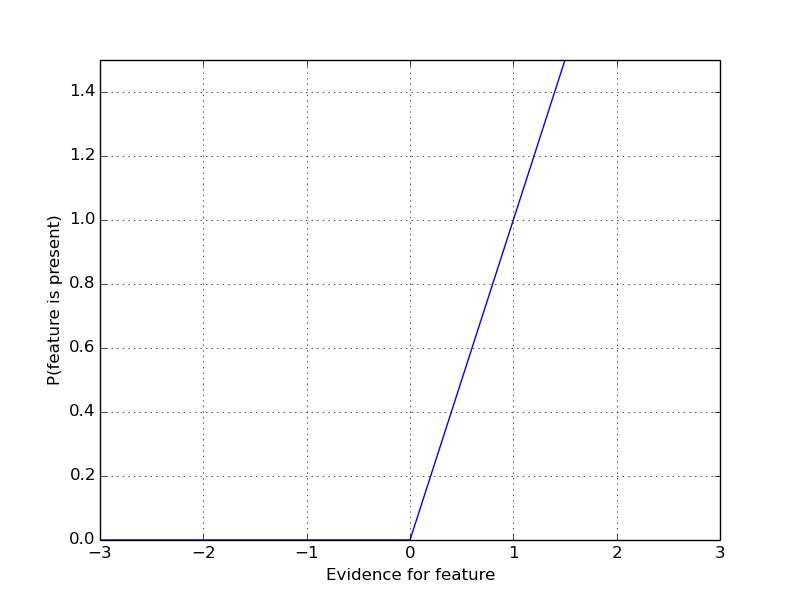
\includegraphics[scale=0.5]{images/ReLU.png}
	\caption{Single-Input Rectified Linear Neuron}
\end{figure}

\paragraph{Softmax Neuron}
\begin{equation}
\label{}
y_{j} = \frac{e^{z_{j}}}{\sum\limits_{i=1}^k e^{z_{i}}} \text{, where } z_{j} = b_{j} + \sum\limits_{i=1}^k x_{i}\cdot w_{i,j}
\end{equation}

The equation of a softmax neuron needs to be understood in the context of a layer of $k$ such neurons within a neural network: therefore, the notation $y_{j}$ corresponds to the output of the $j^{th}$ softmax neuron, and $w_{i,j}$ corresponds to the weight of $x_{i}$ as in input for the $j^{th}$ softmax neuron. A layer of softmax neurons distinguishes itself from others in that neighbouring neurons interact with each other: as can be seen from the equation, the input vectors of all the softmax neurons $z_{1}, z_{2}, ..., z_{k}$ serve to enforce $\sum\limits_{i=1}^k y_{i} = 1$. In other words, the vector $(y_{1}, y_{2}, ..., y_{k})$ defines a probability mass function. This makes the softmax layer ideal for classification: neuron $j$ can be made to represent the probability that the input is an instance of class $j$. Another attractive aspect of the softmax neuron is that its derivative is quick to compute: it is given by $\frac{dy}{dz} = \frac{y}{1-y}$.


\section{Training: Backpropagation}

Now that the architecture of a deep CNN has been explained, the question remains of how to train it. Mathematically: now that the function space has been explained, the question remains of how this space is searched. In the case of feed-forward neural networks and supervised learning, this is done with gradient descent, a local (therefore greedy) optimisation algorithm. Gradient descent relies on the partial derivatives of the error (a.k.a\ cost) function with respect to each parameter of the network; the backpropagation algorithm is an implementation of gradient descent which efficiently computes these values.
  
\subsubsection{Compute Error-Weight Partial Derivatives}

Let $t$ be the target output (with classification, this is the label) and let $y = (y_{1}, y_{2}, ..., y_{P})$ be actual value of the output layer on a training case. (Note that classification is assumed here: there are multiple output neurons, one for each class).

The error is given by 
\begin{equation}
E = \mathcal{C}(\textbf{t}-\textbf{y})
\end{equation}

where $\mathcal{C}$ is the chosen cost function. The error-weight partial derivatives are given by

\begin{equation}
\frac{\partial{E}}{\partial{w_{ij}}} = \frac{\partial{E}}{\partial{y_{i}}} \cdot \frac{\partial{y_{i}}}{\partial{net}} \cdot \frac{\partial{net}}{\partial{w_{ij}}}
\end{equation}

Since in general, a derivative $\frac{\partial{f}}{\partial{x}}$ is numerically obtained by perturbing $x$ and taking the change in $f(x)$, the advantage with this formula is that instead of individually perturbing each weight $w_{ij}$, only the unit outputs $y_{i}$ are perturbed. In a neural network with $k$ fully connected layers and $n$ units per layer, this amounts to $\Theta(k \cdot n)$ unit perturbations instead of $\Theta(k \cdot n^{2})$ weight perturbations (note that the bound on weight perturbations is no longer tight if we drop the assumption of fully connected layers).

\paragraph{How Gradient Propagates}

It is important for intuition to realise how the gradient propagates through a network - especially since a single piece of information - the error - is supposed to adjust up to millions of parameters, which could be considered as a bit of a stretch. Let us note that in the case of classification, the error is not a scalar, but a vector of size equal to the number of classes, so it carries more than "one piece" of information. \\

With the following notation:
\begin{itemize}
\renewcommand\labelitemi{--}
\item $y_{j}$, the output of unit (a.k.a\ neuron) $j$, but also used to refer to the unit $j$ itself
\item $w_{ij}$, the weight of the edge connecting lower-layer neuron $y_{i}$ to upper-layer neuron $y_{j}$
\item $z_{j} := b+ \langle x,w \rangle = b + \sum\limits_{i=1}^k x_{i}\cdot w_{ij}$, the input vector for $y_{j}$ -- therefore $y_{j} = \psi(z_{j})$ \\
\end{itemize}

The rules for propagating the gradient backwards through a network are:
\begin{itemize}
\renewcommand\labelitemi{--}
\item to \textbf{initialise}: $grad \leftarrow \mathcal{C}'(y_{L})$, where $y_{L}$ is the output unit
\item to \textbf{propagate through a unit} $y_{j}$: $grad \leftarrow grad \cdot \psi'(z_{j})$
\item to \textbf{propagate through an edge} $w_{ij}$: $grad \leftarrow grad \cdot w_{ij}$
\item to \textbf{stop at an edge} $w_{ij}$: $grad \leftarrow grad \cdot y_{i}$ \\
\end{itemize}

Note that 

\begin{figure}[h!]
	\centering
	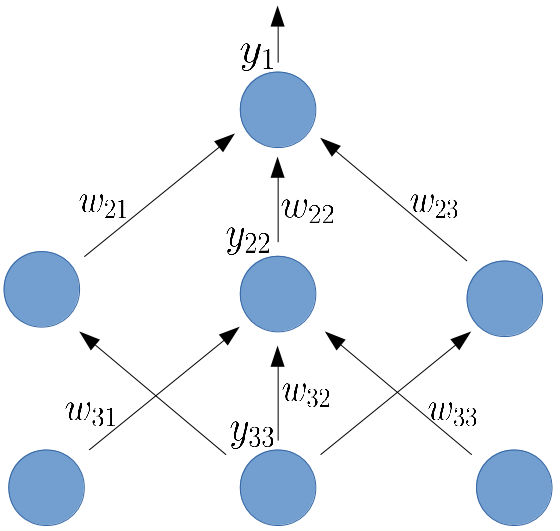
\includegraphics[scale=0.28]{images/gradient_propagates.png}
	\caption{(CHANGE NOTATION to reflect one above with $\textbf{y}_L$ for top layer) Feed-Forward Neural Network with one Hidden Layer}
\end{figure}

So for example, given the figure above:
\begin{itemize}
\renewcommand\labelitemi{--}
\item for $\frac{\partial{E}}{\partial{w_{57}}}$: initialise, propagate through $y_{7}$, then stop at $w_{57}$:
 $ \mathcal{C}'(y_{7}) \cdot \psi'(z_7) \cdot y_5$ 
\item for $\frac{\partial{E}}{\partial{w_{25}}}$: initialise, propagate through $y_{7}$, $w_{57}$, $y_{5}$ then stop at $w_{25}$:
 $\mathcal{C}'(y_{7}) \cdot \psi'(z_7) \cdot w_{57} \cdot \psi'(z_5) \cdot y_2$ \\
\end{itemize}

% took this out of eq above to reduce clutter, but you might need it later on
%\begin{equation}
%\frac{\partial{E}}{\partial{w_{22}}} = \frac{\partial{\mathcal{C}(y_{1})}}{\partial{w_{22}}} = %\frac{\partial{\mathcal{C}(\psi(\sum\limits_{i=1}^k x_{2i}\cdot w_{2i}))}}{\partial{w_{22}}} = \frac{d \mathcal{C}(y_{1})}{dy_{1}} \cdot \frac{d \psi(z_{11})}{dz_{11}} \cdot \frac{\partial{(\sum\limits_{i=1}^k x_{2i}\cdot w_{2i})}}{\partial{w_{22}}}
%\end{equation}


\subsubsection{Update Weight Values (with Stochastic Gradient Descent)}

The learning rule is given by $w_{i,t+1} = w_{i,t+1} + \tau \cdot \frac{\partial{E}}{\partial{w_{i,t}}}$

\begin{figure}[h!]
	\centering
	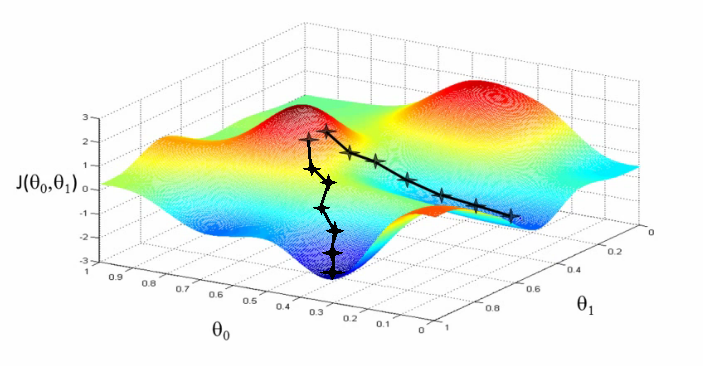
\includegraphics[scale=0.8]{images/local_minima.png}
	\caption{an error surface with poor local minima}
\end{figure}

Visually, this means that weight values move in the direction the will reduce the error quickest, i.e.\ the direction of steepest descent on the error surface is taken. Notice that given the learning rule, gradient descent converges (i.e.\ $w_{i,t+1}$ equals $w_{i,t+1}$) when the partial derivative reaches zero. This corresponds to a local minimum on the error surface. In the figure below, two potential training sessions are illustrated. The minima attained in each cases are not the same. This illustrates a strong shortcoming with backpropagation: parameter values can get stuck in poor local minima.


\begin{thebibliography}{1}
% Example: \bibitem{One}
% a better way of doing it: a .bib file or something. bit.ly/1kqg2Qe
\bibitem{decaf}
 Donahue, Jeff; Jia, Yangqing; Vinyals, Oriol; Hoffman, Judy; Zhang, Ning; Tzeng, Eric; Darrell, Trevor;
  \emph{DeCAF: A Deep Convolutional Activation Feature for Generic Visual Recognition}\\
  arXiv preprint arXiv:1310.1531, 2013

\bibitem{MIML}
 Zhou, Zhi-Hua; Zhang, Min-Ling;
  \emph{Multi-Instance Multi-Label Learning with Application to Scene Classification}\\
  Advances in Neural Information Processing Systems 19, 
  Proceedings of the Twentieth Annual Conference on Neural Information Processing Systems, 
  Vancouver, British Columbia, Canada, 
  December 4-7, 2006

\bibitem{f-measure}
 Pastor-Pellicer, Joan; Zamora-Martinez, Francisco; Espana-Boquera, Salvador; Castro-Bleda, Maria Jose;
  \emph{F-Measure as the Error Function to Train Neural Networks}\\

\bibitem{control-point}
 Fusion Group - ControlPoint LLP,
 \emph{Company Description}\\
 URL: \url{http://www.fusionprovida.com/companies/control-point}, last accessed 5th June 2014. 
  
\bibitem{univ-approx}
 Barron, Andrew R.,
 \emph{Universal Approximation Bounds for Superpositions of a Sigmoidal Function}\\
 IEEE Transactions on Information Theory, 
 Vol. 39, No. 3
 May 1993

\bibitem{DL-book}
 Bengio, Yoshua;
 \emph{Learning Deep Architectures for AI}\\
 Foundations and Trends in Machine Learning, 
 Vol. 2, No. 1 (2009) 1-127
 2009

\bibitem{Russel & Norvig}
 Russell, Stuart J; Norvig, Peter;
 \emph{Artificial Intelligence: A Modern Approach}\\
 2003

\bibitem{krizhevsky}
 Krizhevsky, Alex; Sutskever, Ilya; Hinton, Geoffrey E.;
 \emph{ImageNet Classification with Deep Convolutional Neural Networks}\\
 2012

\bibitem{rectifier}
 Glorot, Xavier; Bordes, Antoine; Bengio, Yoshua;
 \emph{Deep Sparse Rectifier Neural Networks}\\
 2013

\bibitem{MLP-univ-approx}
 Hornik, Kur; Stinchcombe, Maxwell; White, Halber;
 \emph{Multilayer Feed-Forward Networks are Universal Approximators}\\
 1989

\bibitem{office}
 Saenko, K., Kulis, B., Fritz, M., and Darrell, T.;
 \emph{Adapting visual category models to new domains}\\
 ECCV, 2010

\bibitem{surf}
 Bay, H., Tuytelaars, T., and Gool, L. Van;
 \emph{SURF: Speeded up robust features}\\
 ECCV, 2006

\bibitem{transfer-learning}
 Sermanet, Pierre; Eigen, David; Zhang, Xiang; Mathieu, Michael; Fergus, Rob; LeCun, Yann;
 \emph{OverFeat: Integrated Recognition, Localization and Detection using Convolutional Networks}\\
 arXiv:1312.6229
  
\bibitem{f-measure}
 Joan Pastor-Pellicer, Francisco Zamora-Martínez, Salvador España-Boquera, María José Castro-Bleda;
 \emph{F-Measure as the Error Function to Train Neural Networks}\\
 Advances in Computational Intelligence
 Volume 7902, 2013, pp 376-384
 
\bibitem{cuda-convnet}  
 URL: \url{https://code.google.com/p/cuda-convnet/}, last accessed 6th June 2014.

\end{thebibliography}

\end{document}
